\chapter{Sung keyword spotting experiments and results} \label{chap:kws}
Keyword spotting is another task for which the new acoustic models described in chapter \ref{chap:phonerec} were employed. A keyword-filler HMM algorithm was selected due to its independence on phoneme durations, which is a condition that cannot be fulfilled easily in singing. As described in section \ref{sec:tech_kwfhmm}, keyword-filler HMMs consist of two sub-HMMs: One to model the keyword and one to model everything else (=filler). The keyword HMM has a simple left-to-right topology with one state per keyword phoneme. The filler HMM is a fully connected loop of all phonemes. When the Viterbi path with the highest likelihood passes through the keyword HMM rather than the filler loop, the keyword is detected. Keyword detection was performed on whole songs, which is a realistic assumption for many practical applications. The \textit{ACAP} and \textit{DampTest} data sets were used for evaluation with the keyword set described in section \ref{sec:data_kws}. Song-wise $F_1$ measures were calculated for evaluation.

\section{Keyword spotting using keyword-filler HMMs}
\subsection{Comparison of acoustic models}
Phoneme posteriorgrams were generated with the various acoustic models described in section \ref{sec:phonerec_acap}. The results in terms of $F_1$ measure across the whole \textit{DampTest} sets are shown in figure \ref{fig:kws_exp1}. Figure \ref{fig:kws_exp1_acap} show the results of the same experiment on the small \textit{ACAP} data set.

Across all keywords, a document-wise $F_1$ measure of $0.35$ is obtained using the posteriorgrams generated with the \textit{TIMIT} model on the \textit{DampTest} data sets. This result is slightly higher for the \textit{TimitM} models trained on ``songified'' speech, and rises to $0.45$ using the model trained on the small \textit{DampBB\_small} singing data set. Surprisingly, the model trained on \textit{DampBB} is only slightly better than the much smaller one. Using the very big \textit{DampB} training data set, the $F_1$ measure reaches $0.47$. 

On the hand-annotated \textit{ACAP} test set, the difference is even more pronounced, rising from $0.29$ for the \textit{TIMIT} model to $0.5$ for \textit{DampB}. This might, again, be caused by the more accurate annotations or by the higher-quality singing. Additionally, the data set is much smaller with fewer occurrences of each keyword, which could emphasize both positive and negative tendencies in the detection.

%TODO: recall vs. precision -> �berleitung zu duration modeling


\begin{figure}
        \centering
        \begin{subfigure}[t]{0.4\textwidth}
		 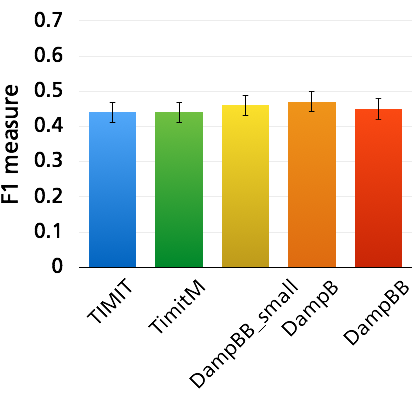
\includegraphics[width=\textwidth]{images/kws_exp1.png}
                \caption{$F_1$ measures for keyword spotting results on the \textit{DampTest} data sets.}
                \label{fig:kws_exp1}

        \end{subfigure}%
        \hfill
         %add desired spacing between images, e. g. ~, \quad, \qquad, \hfill etc.
          %(or a blank line to force the subfigure onto a new line)
        \begin{subfigure}[t]{0.4\textwidth}
                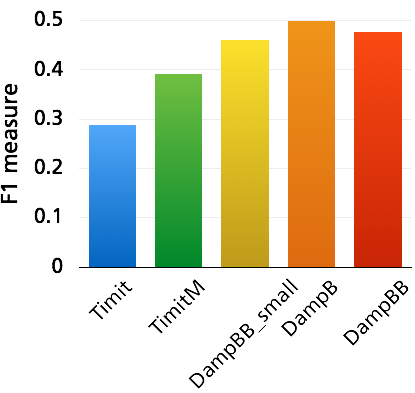
\includegraphics[width=\textwidth]{images/kws_exp1_acap.png}
                \caption{Keyword spotting results on the \textit{ACAP} data set.}
                \label{fig:kws_exp2}
        \end{subfigure}
        \caption{$F_1$ measures for keyword spotting results using posteriorgrams generated with various acoustic models.}
          \end{figure}
%\vspace{-5px}

\subsection{Gender-specific acoustic models}
%TODO: ACAP??
Keyword spotting was also performed on the posteriorgrams generated with the gender-dependent models trained on \textit{DampF} and \textit{DampM} (also described in section \ref{sec:phonerec_acap}. The results are shown in figure \ref{fig:kws_exp2}.

In contrast to the phoneme recognition results from Experiment C, the gender-dependent models perform slightly better for keyword spotting than the mixed one of the same size, and almost as good as the one trained on much more data (\textit{DampB}). The $F_1$ measures for the female test set are  $0.48$ for the \textit{DampB} model, $0.45$ for the \textit{DampBB} model, and $0.46$ for the \textit{DampFB} model. For the male test set, they are $0.46$ and $0.45$ for the first two, and $0.46$ for the \textit{DampMB} model.



\subsection{Individual analysis of keyword results}
%TODO: ACAP??
Figure \ref{fig:kws_exp3} shows the individual $F_1$ measures for each keyword using the best model (\textit{DampB}), ordered by their occurrence in the \textit{DampTest} sets from high to low (i.e. number of songs which include the song). There appears to be a tendency for more frequent keywords to be detected more accurately. This happens because a high recall is often achievable, while the precision depends very much on the accuracy of the input posteriorgrams. The more frequent a keyword, the easier it also becomes to achieve a higher precision for it.

As shown in literature \cite{phdthesis:thambiratnam}, the detection accuracy also depends on the length of the keyword: Keywords with more phonemes are usually easier to detect. This might explain the relative peak for ``every", ``little", and ``always", in contrast to ``eyes" or ``world". Since keyword detection systems tend to perform better for longer words and most of the keywords only have 3 or 4 phonemes, this result is especially interesting.

One potential source of error are sequences of phonemes that overlap with keywords, but are not included in the calculation of the precision. Words spelled the same were included, but split phrases or other spellings were not (e.g. ``away" as part of ``castaway" would be counted, but ``a way" would not be counted as ``away"). This might artificially lower the results and could be an avenue for future improvement. Additionally, only one pronunciation for each keyword was provided, but there may be several possible.

\setlength{\belowcaptionskip}{-10pt}
\begin{figure}
 \begin{center}
                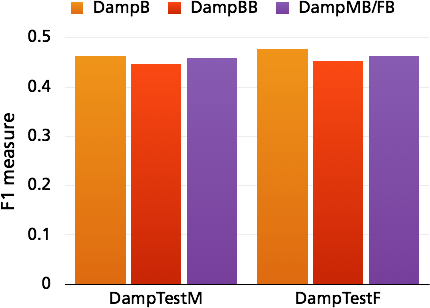
\includegraphics[width=0.5\textwidth]{images/kws_exp2.png}
                \caption{$F_1$ measures for keyword spotting results on the \textit{DampTestM} and \textit{DampTestF} data sets using mixed and gender-dependent models.}
                \label{fig:kws_exp2}
                 \end{center}
 \end{figure}

\begin{figure}
 \begin{center}
                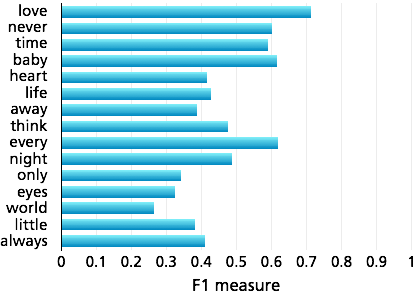
\includegraphics[width=0.5\textwidth]{images/kws_exp3.png}
                \caption{Individual $F_1$ measures for the results for each keyword, using the acoustic model trained on \textit{DampB}.}
                \label{fig:kws_exp3}
                 \end{center}
 \end{figure}
%\vspace{-5px}





\section{Keyword spotting using duration-informed keyword-filler HMMs}
As mentioned above, a high recall is easily achievable with the described approach, but the comparatively low precision decreases the over-all result. Therefore, using additional information to sort out false positives would be a helpful next step.\\
One such source of information are the durations of the detected phonemes. As shown in figure \ref{fig:phone_durations}, each phoneme in the \textit{TIMIT} speech database has a fairly fixed duration. In singing, the vowels' durations vary a lot, but the consonants' are still quite predictable. Standard HMMs do not impose any restrictions on the state durations, resulting in a geometric distribution which does not correspond to naturally observed phoneme durations. \\
As first described in \cite{ferguson}, introducing restrictions on state durations can improve the recognition results. In \cite{juang}, Juang et al. present two basic approaches for duration modeling in HMMs: Internal duration modeling and Post-processor duration modeling.\\

In internal duration modeling, the durations are incorporated directly into the Viterbi alignment. This means that the Viterbi output will already be a state sequence that is optimal with regards to the a-priori phoneme duration knowledge. It is, however, computationally expensive. In previous experiments \cite{kruspe_kws2}, this approach did not produce better results than the much easier to implement post-processor duration modeling. Therefore, this section will focus on that approach.\\

When using post-processor duration modeling, knowledge about plausible phoneme durations is imposed on the result of the Viterbi alignment, the obtained state sequence. This is computationally cheap, but only results in a new likelihood score for the obtained sequence and does not provide better possible state sequences. The state sequence obtained from the Viterbi alignment is afterwards re-scored as described in section \ref{sec:tech_duration_modeling}, and all occurrences of the keyword with a score below a certain threshold are discarded.



%TODO: clean up
\section{Conclusion}\label{sec:kws_conclusion}
%insgesamt besser
%huge DampB set best, but 3% DampBB almost as good
% even v small DampBB_small better than Timit
% context does not help
% gender models slightly better for kws, not better for phone rec --> variability?
% results phonerec
% results kws - esp. interesting because short
%---auto alignment error source

In this paper, we trained new acoustic models on a large corpus of unaccompanied singing recordings. Since no annotations for these existed, we first had to automatically align lyrics to them. The new models could then directly be trained on these automatic annotations. To our knowledge, this has not been done before for singing.

We trained three different models with mixed gender recordings: One on 6000 full recordings of 301 songs, one on just 4\% of this data, and one which was balanced by phonemes and is roughly half the size of the medium-sized one. We then tested their performance on two other subsets of the same corpus which did not overlap with the training data, and on a small unrelated data set of commercial vocal tracks which were hand-annotated.

In all cases, the three new models showed a strong improvement over those trained only on speech. Even the model trained on the smallest set produced a jump in correctly classified frames from $13\%$ to $19\%$, and in weighted phoneme error rate from $0.9$ to $0.77$ on the large test set. With the model trained on the medium-sized data set, we obtained $23\%$ correct frames and a weighted phoneme error rate of $0.65$. With the biggest one, the weighted phoneme error rate falls to $0.6$. The results are similar on the small hand-annotated test set.

We also tested acoustic models with 8 context frames, and models trained on gender-specific data. Neither of them showed improvement over the first ones.

We then performed keyword spotting for 15 keywords on phoneme posteriorgrams generated with these new models using a keyword-filler approach. The resulting $F_1$ measure rises from $0.35$ for the models trained on speech to $0.47$ for our new models. This result is especially interesting because most of the keywords have few phonemes. For keyword spotting, gender-dependent models perform slightly better than mixed-gender models of the same size.

%\vspace{-5px}

\section{Future work}\label{sec:future}
%plp?
%other feats?
%find out where exactly improvement ends
%full recordings - maybe reduced set?
% pronunciation variants
%language modeling
%alignment works well - 
%combine with textual information?
%phrase spotting
%bigger models
%use on polyphonic data
% maybe specific sets/keywords/styles/applications?
So far, we have only tested this approach using MFCC features. As shown in our previous experiments \cite{kruspe_kws1}, other features like TRAP or PLP may work better on singing. So-called log-mel filterbank features have also been used successfully with DNNs \cite{hinton}. Another interesting factor is the size and configuration of the classifiers, of which we have only tested one so far. Since the alignment appears to provide valid training data, we believe the features and model configuration could be the greatest sources of improvement.

We showed that there is only a slight amount of improvement between the model trained on all 6000 songs and the one trained only on $4\%$ of this data. It would be interesting to find the exact point at which additional training data does not further improve the models. On the evaluation side, a keyword spotting approach that allows for pronunciation variants or sub-words may produce better results. Language modeling might also help to alleviate some of the errors made during phoneme recognition.

These models have not yet been applied to singing with background music, which would be interesting for practical applications. Since this would probably decrease the result when used on big, unlimited data sets, more specified systems would be more manageable, e.g. for specific music styles, sets of songs, keywords, or specialized applications. Searching for whole phrases instead of short keywords could also make the results better usable in practice.

As shown in \cite{mesaros_alignment} and \cite{goto_alignment}, alignment of textual lyrics and singing already works well. A combined approach that also employs textual information could be very practical.